Mapping is the process of finding the location in the reference genome where a DNA read from a sample probably belongs to. Since 99\% of the genome is the same in a species, finding the location in the reference genome is similar to identify the position of a read in the sample DNA. Moreover, the mapping must also provide the information about how well the read is aligned to the reference genome giving the exact location and nature of each kind of mutation (insertion, deletion or modification of one or multiple bases).  Mapping DNA reads is a complex task due to large sequencing data and reference genome size. Different types of mutations also increase the complexity of the mapping. In the case of the human, we can write the whole sequence of nucleotides with A, T, C, and G letters, just like a long string of characters. If each character is encoded on a byte, the whole text would be around 3.4GB. Even though it seems small regarding today's standards of data storage, looking for a particular area that would match a string is far from trivial. As such, a sophisticated way to look into the genome and find an alignment is needed.


At the moment, DNA mapping represents the first genomics analysis step of many DNA analysis approaches in practice. The complicated process of DNA mapping is rather time consuming, both due to the high complexity of the analysis involved as well as the amount of data that needs to be processed. In many cases, mapping can take between $30\%$ and $50\%$ of the total DNA analysis time. Figure~\ref{fig:pipelineprocesstime} shows that the time taken by mapping which is about a third of the total pipeline time. Moreover, the time taken for this part is counted in thousands of CPU-core hours for this example data set. Therefore DNA mapping is a computational challenge and various techniques to achieve it in a timely manner. The problem at stake is then to find an effective way to compute DNA alignment as fast as possible.

\begin{figure}[h]
	\centering
	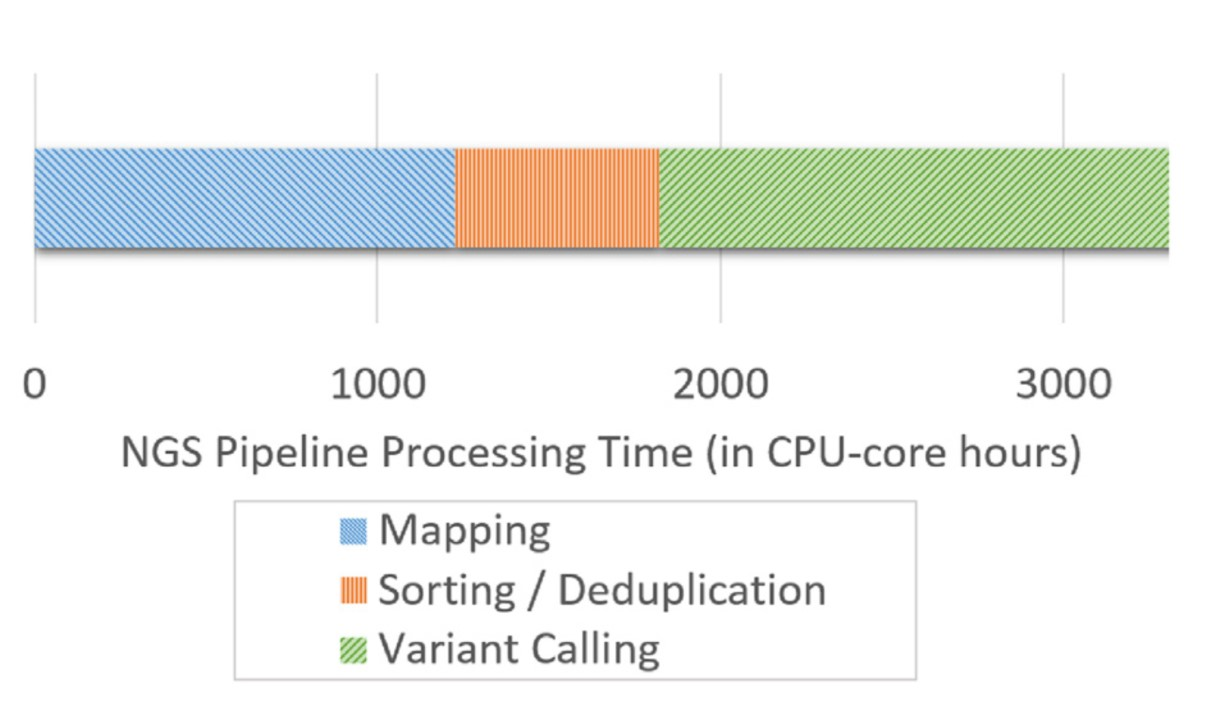
\includegraphics[width=1\linewidth]{pipelineprocesstime}
	\caption{DNA pipeline process time share for a typical 30$\times$ coverage cancer DNA data set. The data set consists of three tumor samples and one normal tissue sample (time given in CPU-core hours). (from~\cite{HOUTGAST201854})}
	\label{fig:pipelineprocesstime}
\end{figure}


% refer to that paper : https://www.sciencedirect.com/science/article/pii/S1476927118301555 and also show the figure in the paper (copy it and use a reference)
